\documentclass{beamer}

\usepackage[utf8]{inputenc}
\usepackage{bm}
\usepackage{mathrsfs}
\usepackage[]{graphicx}
\usepackage[]{color}
\usepackage{geometry}
\usepackage{soul}


\usepackage{multimedia}







%Information to be included in the title page:
\title{\textcolor{white}{Physics of
\\ Lumen Formation and Interaction}}
\author{\textcolor{white}{Godwin Martin}}
\date{}


\begin{document}
\beamertemplatenavigationsymbolsempty
\setbeamertemplate{background}{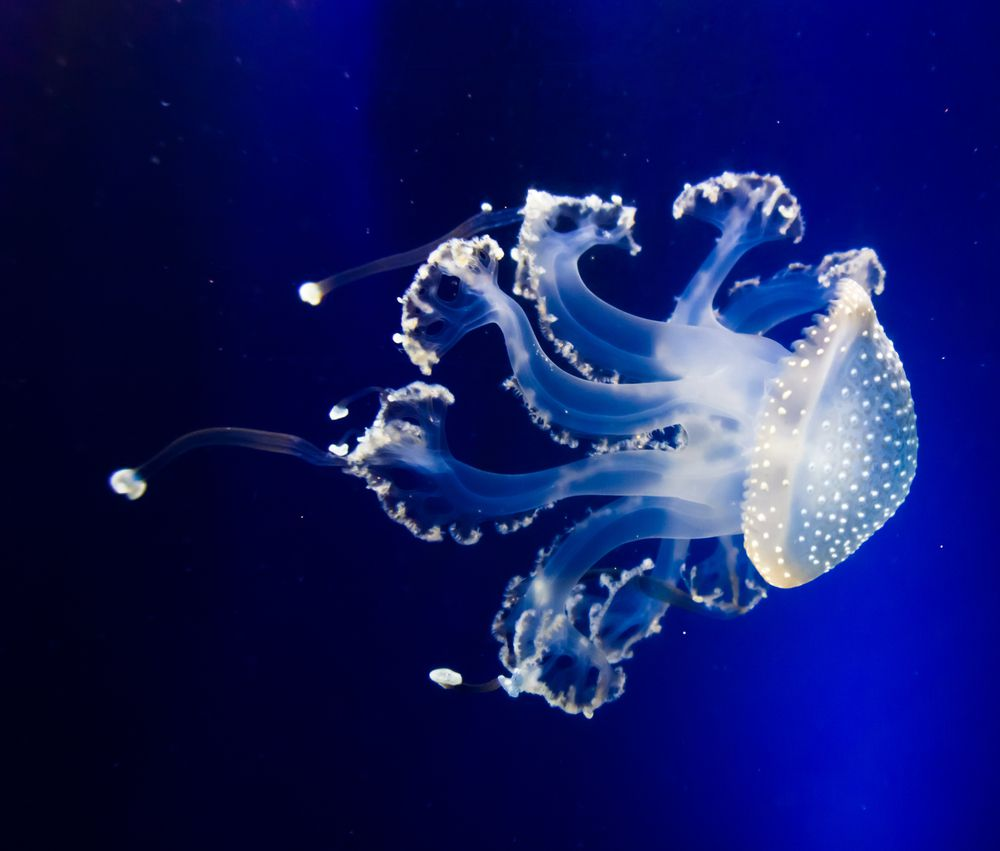
\includegraphics[width=\paperwidth,height=\paperheight]{jellyfish.jpg}}
\frame{\titlepage}









\setbeamertemplate{background}{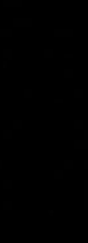
\includegraphics[width=\paperwidth,height=\paperheight]{black.png}}
\begin{frame}
\frametitle{\textcolor{white}{How do living beings form tubes and cavities?}}

\begin{figure}
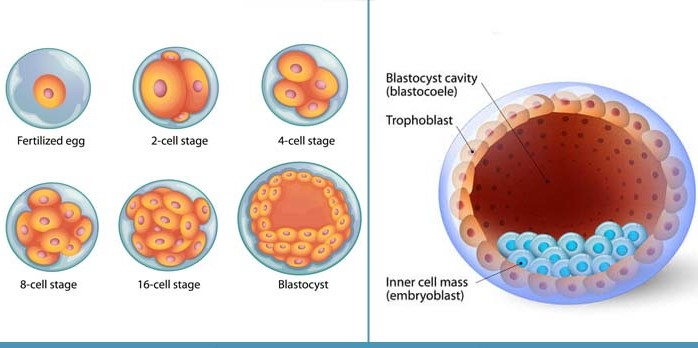
\includegraphics[scale=0.5]{blastocyst.jpg}
\end{figure}


\end{frame}




















\begin{frame}{\textcolor{white}{What are the possible mechanisms?}}

\textcolor{blue!50!green!20}{$\bullet$ Coarsening}


\begin{figure}
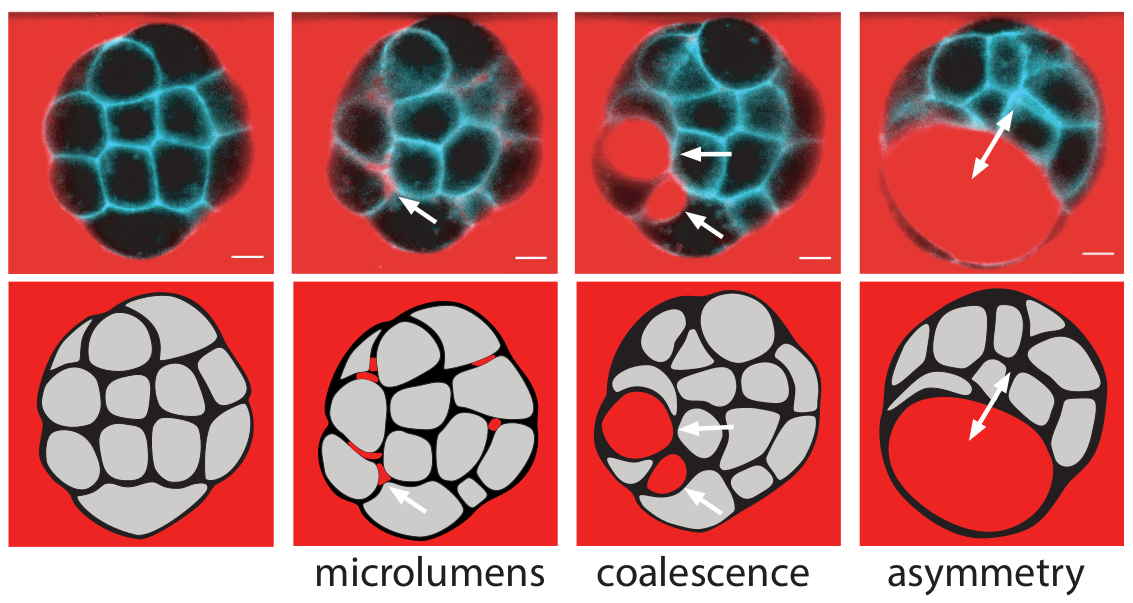
\includegraphics[scale=0.20]{coarsening.png}
\end{figure}

\textcolor{blue!50!green!20}{$\bullet$ Fluid Pumping}\\
\ 
\\

\textcolor{blue!50!green!20}{$\bullet$ Electrostatic Interactions}




\end{frame}


\begin{frame}
\frametitle{\textcolor{white}{Fluxes of water and solutes}}

\begin{figure}
\centering
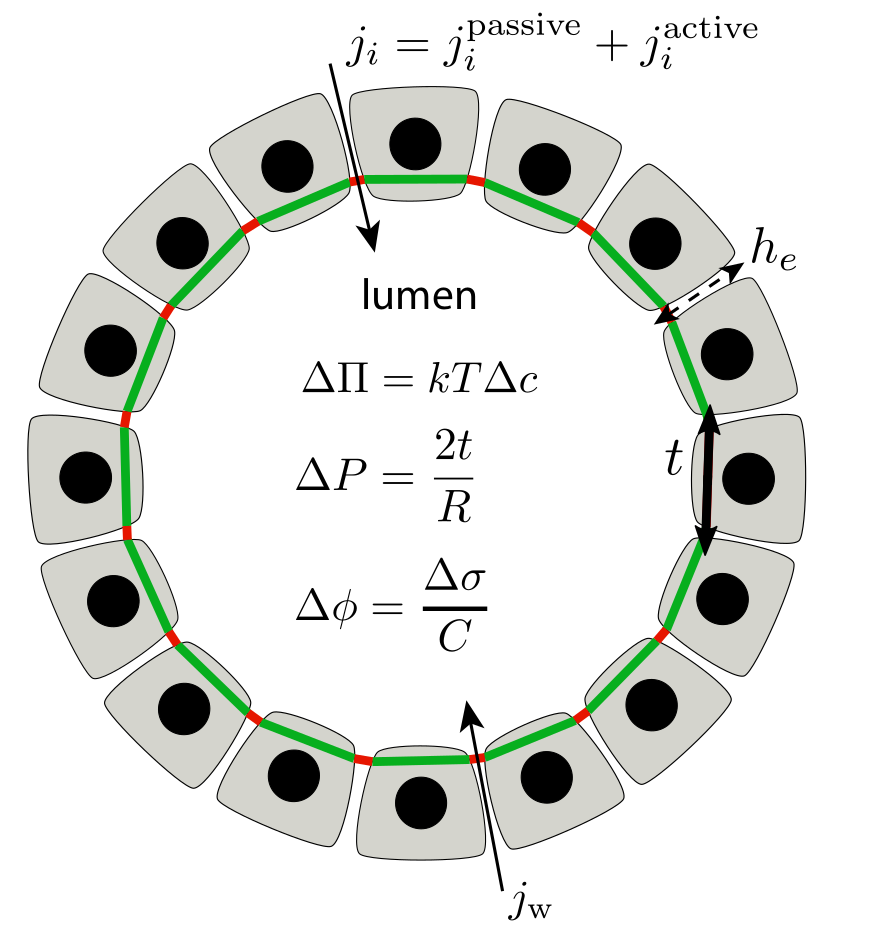
\includegraphics[scale=0.2]{tissue_pumping.png}
\end{figure}
\end{frame}





\begin{frame}
\frametitle{\textcolor{white}{Fluxes of water and solutes}}

\textcolor{blue!50!green!20}{Say there are $N$ ionic solutes and the $i^{th}$ solute has a charge $q_i$}

\textcolor{white}{
\begin{equation}
j_w = \lambda _w (\textcolor{blue!50}{\Delta \Pi} - \Delta P) - \sum_{i=1}^{N}\lambda_{w,i} \left(\Delta c_i + \frac{q_i \overline{c_i}}{k_B T} \textcolor{red!30}{\Delta \phi}\right) + j_{w}^{active}
\end{equation}
\begin{align*}
j_i &= - \lambda_i \left(\Delta c_i + \frac{q_i \overline{c_i}}{k_B T} \textcolor{red!30}{\Delta \phi}\right) + \lambda_{i,w} (\textcolor{blue!50}{\Delta \Pi} - \Delta P)\\ 
 & \quad \quad \quad \quad - \sum_{j \neq i} \lambda_{i,j} \left(\Delta c_j + \frac{q_j \overline{c_j}}{k_B T} \textcolor{red!30}{\Delta \phi}\right) + j_i ^{active}
\end{align*}}


\textcolor{blue!50}{Osmotic Pressure}, \textcolor{red!30}{Electric Potential}

\end{frame}



\begin{frame}{\textcolor{yellow!10!blue!50!white!50}{Osmotic pressure plays a big role in forming lumens}}
\textcolor{white}{
\begin{align*}
j_w = \lambda_w (\Delta \Pi - \Delta P)
\end{align*}
\\
For MDCK cells,
\begin{equation*}
\lambda_w \sim (0.1-1) \times 10^{-7} \mu m s^{-1} Pa^{-1}
\end{equation*}
During growth of the zebrafish inner ear
\begin{equation*}
j_w \sim 1-8 \mu m /h
\end{equation*}
This gives
\begin{equation*}
\Delta \Pi - \Delta P \sim 3 - 200 kPa
\end{equation*}
Direct measurements $\implies$
\begin{equation*}
\Delta P \sim 100-300 Pa
\end{equation*}
}
\end{frame}






\begin{frame}{\textcolor{yellow!10!blue!50!white!50}{Active pumps are crucial in lumen formation\\
No pumps, no lumen}}

\begin{figure}
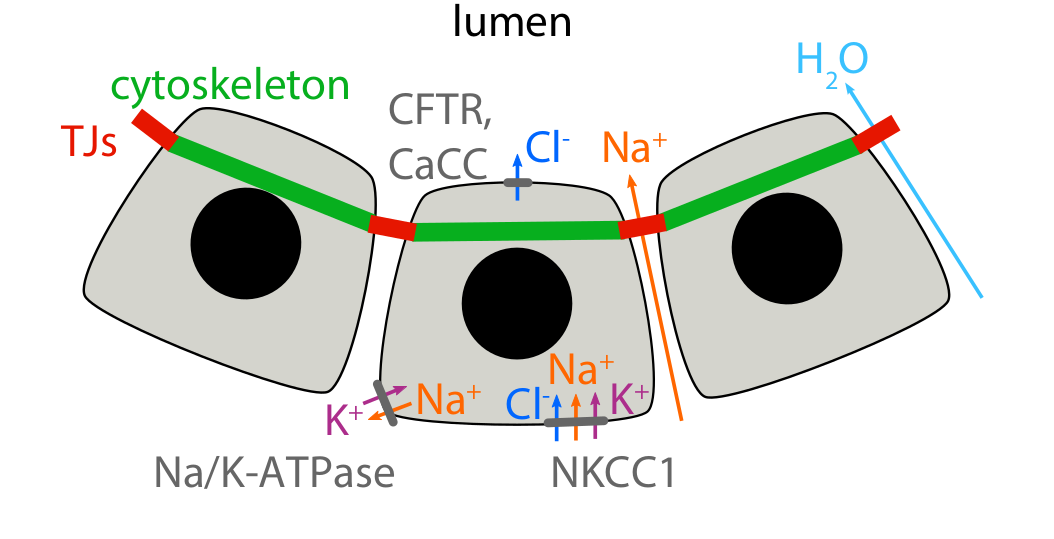
\includegraphics[scale=0.2]{active.png}
\end{figure}

\textcolor{white}{Inhibition of Na/K-ATPase pump blocks lumen formation.}

\textcolor{blue!20}{Doesn't end there. Primary channels are followed by secondary channels. Therefore, a massive contribution.}
\end{frame}




\begin{frame}{\textcolor{yellow!10!blue!50!white!50}{Spherical \st{Cow} Lumen}}


\textcolor{white}{
\begin{align*}
\dot{R} &= \lambda_w (\Delta \Pi - \Delta P)\\
\frac{R}{3} \dot{c_i^{\ell}} &= -\dot{R} c_i^{\ell} - \lambda_i [\Delta c_i + \frac{q_i \overline{c_i}}{k_B T} \Delta \phi] + j_i^{active}
\end{align*}
Where
\begin{align*}
\Delta \phi &= \frac{R}{6C} \sum_{i} q_i \Delta c_i\\
\Delta \Pi &= k_B T \sum_i \Delta c_i\\
\Delta P &= \frac{2t}{R}
\end{align*}
}
\end{frame}




\begin{frame}{\textcolor{yellow!10!blue!50!white!50}{How do smaller lumens form bigger lumens?}}
\begin{center}
\movie[height = 0.4\textwidth, width = 0.6\textwidth, poster, showcontrols] {}{aaw7709s7.mov}
\end{center} 


\end{frame}


\begin{frame}{Pump-leak mechanism}
\textcolor{white}{
$\bullet$ anion of charge $-e$, conc. $c_-$ pumped into lumen with $j^{active}$\\
$\bullet$ cation of charge $e$, con. $c_+$ diffuses passively\\
Lumens needn't be perfectly sealed to grow.
}
\end{frame}




\begin{frame}{\textcolor{yellow!10!blue!50!white!50}{How do smaller lumens form bigger lumens?}}


\begin{center}
\movie[height = 0.6\textwidth, width = 0.8\textwidth, poster, showcontrols] {}{Laplace_pressure.vp9.webm}
\end{center} 
\end{frame}


























\begin{frame}
\frametitle{\textcolor{white}{Can we predict the time scale of coarsening?}}

\textcolor{white}{
\begin{align*}
\mathbf{v}^f = \mathbf{v}^c + \frac{\nabla P^f}{\kappa}
\end{align*}
}
\end{frame}


\begin{frame}{\textcolor{yellow!10!blue!50!white!50}{Nonspherical \st{cows} lumens}}

\end{frame}


\begin{frame}{\textcolor{yellow!10!blue!50!white!50}{So, what have we learnt?}}
\textcolor{green!40!yellow!20!blue!20}{Several mechanisms of lumen formation\\
Fluxes due to osmotic and hydrostatic pressures, chemical and electric potential differences.
}

\end{frame}



\end{document}



\begin{frame}{\textcolor{yellow!10!blue!50!white!50}{Ion permeability of the epithelium}}
\textcolor{white}{
$\lambda_i$ and $\lambda_{w,i}$ include the effects of ion channels, pores, symporters.\\
Measures of $\lambda_i$ are scarce in the literature.\\ We can estimate its order of magnitude.
}
\end{frame}